\chapter{Palabras nuevas}
% Intro {{{
En el capítulo anterior se mencionó que el algoritmo toma como  idioma
influyente a aquel que transmite palabras hacia los demás y que estas perduren
en los receptores al menos dos años.   El objetivo ahora es identificar qué
idioma es más influyente sobre los demás, sin embargo establecer un método que
proporcione este resultado no es sencillo,  puede ser ambiguo decir que algo es
influyente, no hay una manera de seguir una serie de pasos que finalicen en
decir si algo es influyente o no,  o cuánta influencia se tuvo en el proceso.
Incluso que un idioma transmita palabras no es criterio suficiente para afirmar
una influencia.  

Al tener una base de datos  con los préstamos de un idioma en otro,  una primer
manera de establecer la influencia es  identificar los tiempos donde ocurren
las migraciones.  Para ello conviene hacer una clasificación dentro de los
propios préstamos y a partir de ella  continuar con una cuantificación de la
influencia.  Si se tiene una pareja de idioma origen \textit{A} e idioma
receptor \textit{B} entonces se clasifican a los préstamos de \textit{A} en
\textit{B} como:

\textbf{Préstamos Nuevos}: Son palabras que aparecen por primera vez en las más
usadas del idioma \textit{B}.  Únicamente serán nuevos en el primer año de
aparición,  es fundamental tener certeza del año en que ocurrió la migración. 

Se recuerda que todos los préstamos nuevos, volvieron a aparecer en alguna
lista del idioma B posterior al primer año de la migración, omitiendo a
aquellos que solo aparecieron una vez. 

Entonces dentro de los años comprendidos en el conjunto de búsqueda
(1901-2009), existen múltiples posibilidades con las cuáles trabajar a los
cinco idiomas. La manera en que se tratara de llegar a un resultado que muestre
la influencia puede ser de tres formas:
\begin{enumerate}
\item Contando por cada año los préstamos de origen A que están presentes en
los diferentes receptores.
\item Tomar ahora a \textit{A} como el idioma receptor, y contando cuántos
préstamos nuevos de los diferentes orígenes están presentes en cada año. 
\item Tomando fijos un idioma \textit{A} y un idioma \textit{B},  contabilizar
cuántos préstamos nuevos por año se encuentran si se toma a \textit{A} como
origen y a \textit{B} como receptor,  una vez hecho esto  repetir el conteo
intercambiando a \textit{B} como el origen y a \textit{A} como el receptor. 
\end{enumerate}


En los tres casos la influencia estará ligada a la cantidad de préstamos
nuevos.  Las tres formas son correctas y servirán para decir en cual idioma
receptor  el origen \textit{A} ha sido más influyente por haber mayor cantidad
de migraciones; también cuál ha sido el idioma  que más ha influido en
\textit{A} y finalmente entre dos idiomas,  cuál ha influenciado más al otro. 
% }}}
\section{Eventos que ayudan a las migraciones} % {{{

Una parte complementaria de interpretar la influencia es responder qué es lo
que propicia el haber migraciones de un lado hacia otro.  El tener los
préstamos nuevos clasificados por el año de la primera migración ayuda a
identificar posibles causas de carácter histórico que propiciaron las
migraciones en ese año o alrededor de él.  Por ejemplo, la globalización en los
años recientes ha propiciado que una ola de palabras de su campo semántico
hayan migrado entre orígenes y receptores,  \textit{internet},
\textit{computadora}, \textit{web}, \textit{email},  \textit{software}, son
ejemplos de palabras que surgieron tras el fenómeno de globalización. 

Los eventos pueden ser de diferentes tipos y al tratar con idiomas, se espera
que en tales eventos participen países, personajes o  comunidades que hablan
las lenguas involucradas.  El asociar sucesos con palabras y a la vez con
determinados grupos ayudará a mostrar el alcance que tuvo un lenguaje y la
forma en la que surgió la influencia y esta se propagó. 

Como el conjunto de búsqueda abarca 109 años,  la propagación de las palabras
no es inmediata, en diferentes épocas las migraciones ocurrieron de distintas
formas,  por ejemplo, en 1900 la información no circulaba tan rápido como se
hace actualmente, un evento de esta época puede tener repercusiones en cinco,
diez o más años,  dependiendo de factores geográficos, económicos, tecnológicos
y  la  propia relevancia del evento en las demás comunidades.

En cada resultado posterior, se hizo una investigación histórica de las
palabras que conforman los préstamos nuevos entre idiomas,  en la mayor parte
de los casos se ubicaron sucesos para explicar el por qué ciertas palabras
migraron y la importancia del año o años en que lo hicieron. 

% }}}
\section{Búsqueda y lectura de palabras nuevas} % {{{

Ya establecida la forma en que se buscarán  palabras nuevas en los diferentes
idiomas,  los resultados encontrados se presentarán de la siguiente manera:
\begin{itemize}
\item Por cada idioma se determinó la influencia que esté ejerció en los demás,
mencionada en el punto 1 al comienzo del capítulo.   Ya que se el proceso fue
para todos los idiomas,  al ver primero la influencia de \textit{A} sobre
\textit{B}  (y los demás),  en el siguiente resultado se estará cubriendo la
influencia  de \textit{B}  sobre \textit{A} , cubriendo así el punto 2. 
\item La cuantificación de la influencia por los préstamos nuevos se realizó en
el periodo de 109 años (1900 - 2009) y por cada década comprendida en estos
años, es decir por una parte se mostrarán la cantidad de palabras que
aparecieron en los 109 años y por otra parte como se distribuye esta cantidad
en las diferentes décadas.  La intención de este punto es observar en qué
periodos un idioma aportó (recibió) más  hacia (de) los demás.
\item Se proporcionará en \cite{prestamos_nuevos} las listas  de préstamos
nuevos entre cada idioma, agrupados por el año de aparición en el receptor.  Se
especificará en el Anexo 1  la forma de leer e interpretar estas listas.
\item En cada resultado mostrado se agregara un resultado general para la
influencia en los 109 años, y un contexto detallado entre las migraciones hacia
un idioma receptor por década,  enfatizando los sucesos históricos de las
palabras involucradas, así como los posibles detonantes que propiciaron los
movimientos. 
\item Cada análisis tendrá comentarios sobre el punto 3,  las gráficas
correspondientes se anexaran en el apéndice 1.
\end{itemize}

\subsection*{Lectura de las gráficas} % {{{

Para las gráficas del trabajo se utilizaron diferentes colores para
caracterizar las influencias de un idioma, además en cada gráfica se especifica
los idiomas que intervienen y para su mejor lectura se utilizaron
abreviaciones. Los colores y abreviaciones de cada idioma son:

\fxnote{Porfa aprende a hacer tablas, y haz una tabla acá}

inglés   $\,\,\,\,\,\, \rightarrow \,\,\,$   EN   $\,\,\,\rightarrow\,\,\,$  azul

francés  $\,\,\,       \rightarrow \,\,\,$   FR   $\,\,\,\rightarrow\,\,\,$  amarillo

alemán   $\,\,\,       \rightarrow \,\,\,$   GE   $\,\,\,\rightarrow\,\,\,$  violeta

italiano $\,\,          \rightarrow \,\,\,$  IT   $\,\,\,\,\,\rightarrow\,\,\,$  verde

español  $\,\,\,       \rightarrow \,\,\,$  SP   $\,\,\,\rightarrow\,\,\,$  guinda



En cada grafica se especificará por medio de  abreviaciones y  colores a los
idiomas tratados, todo ello en una leyenda; la primera abreviación que será el
idioma origen de los préstamos, y la segunda corresponderá al idioma receptor,
por ejemplo  la leyenda EN-FR serán los préstamos que van del inglés al
francés, en cambio FR-EN son los préstamos que van en sentido contrario

En todas las gráficas, el eje horizontal está representado por los años del
conjunto de búsqueda 1900-2009,  mientras que en el eje vertical se presenta la
cantidad de prestamos nuevos. 
% }}}
% }}}
\section{Palabras nuevas de un idioma en los demás} % {{{
\subsection{Inglés} % {{{

\begin{figure} % {{{
	\begin{center}
		\begin{subfigure}
			[Inglés por siglo.]{
			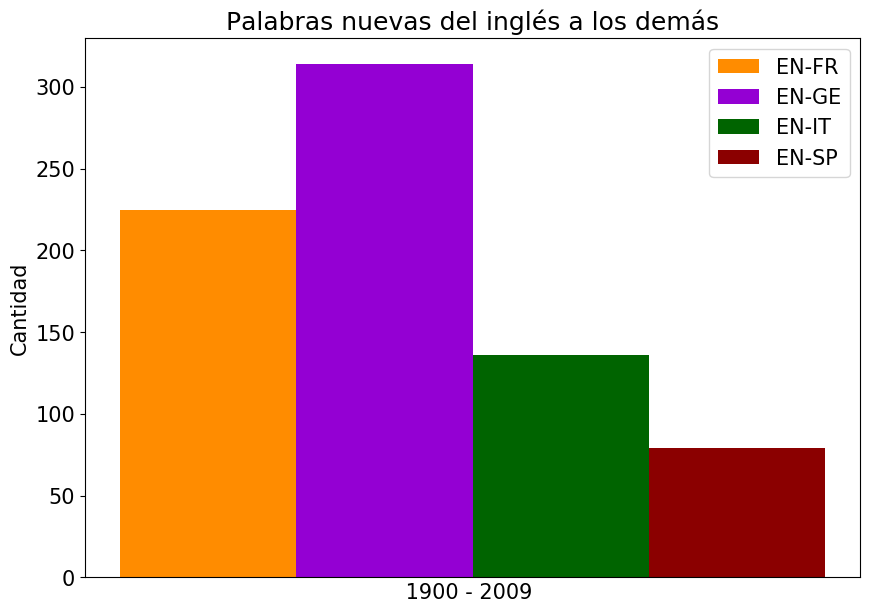
\includegraphics[scale=.4]{Cap_3/ICS_a_EN.png}
			\label{fig.ICS_a_EN}}
		\end{subfigure}
	
	\vspace{0.5cm}
	
		\begin{subfigure}
			[Inglés por década.]{
			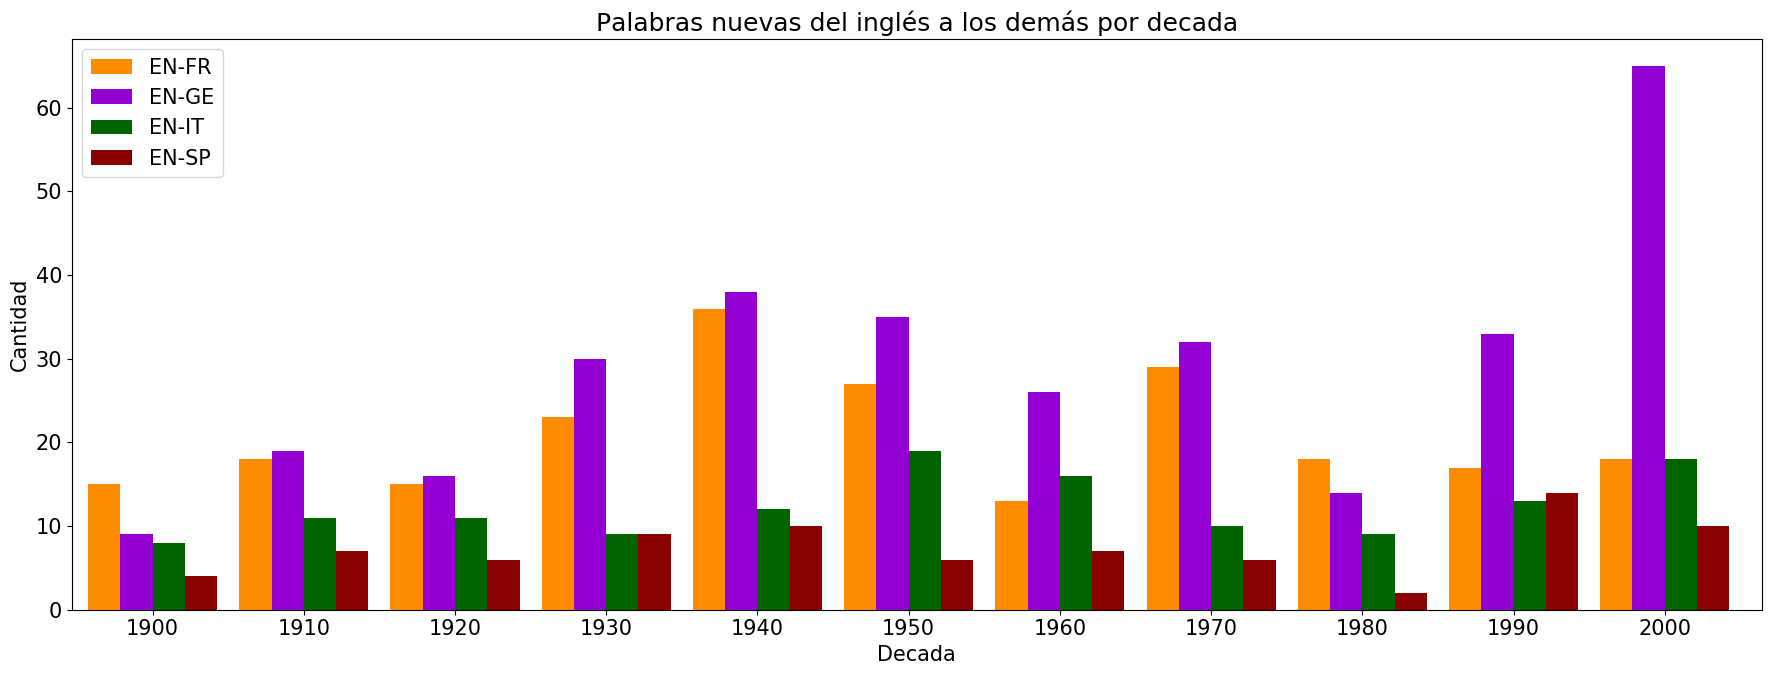
\includegraphics[width=14cm, height=7cm]{Cap_3/ICD_a_EN.png}
			\label{fig.ICD_a_EN}}
		\end{subfigure}
	
	\caption{Palabras nuevas del inglés en los demás.}
	\label{fig.IC_EN}
	\end{center}
\end{figure} % }}}

De manera general, el idioma que más se ha beneficiado del inglés ha sido el
alemán, con 300 préstamos en 100 años.  Inglés y alemán forman parte de la
misma familia lingüística de las lenguas germánicas,  posible razón de los
mayores intercambios. Entre las lenguas romances, el francés fue el más
favorecido, pero también es la más similar por las relaciones normandas entre
ambas.
\subsubsection*{Inglés-Francés} % {{{

Los mayores aportes se dieron de 1930 a 1970, periodo que engloba comienzos de
la gran depresión, la segunda guerra mundial y la guerra fria, sucesos donde
participaron países de ambas lenguas. Las palabras involucradas en este periodo
hacen referencia a estos eventos, entre 1944 y 1945 surgieron en el francés los
términos \textit{Churchill}, \textit{territories}, \textit{nazis} y
\textit{catastrophe},  mientras que en las décadas entre 1950 y 1970
aparecieron \textit{Nixon}, \textit{dollar} y \textit{Johnson}; dos de estas
palabras aluden a apellidos de presidentes de los Estados Unidos,  Lyndon B.
Johnson y Richard Nixon, cuyos periodos de gobierno fueron  entre 1963-1969 y
1969-1974 respectivamente.
% }}}
\subsubsection*{Inglés-Alemán} % {{{
Entre todas las décadas, solo en dos de ellas (1900  y 1980) el alemán no fue
el idioma que mas prestamos recibió  del ingles. Entre las palabras encontradas
en las demás épocas están \textit{economic} (1929), \textit{depression} (1931),
\textit{investment} (1933), \textit{Roosevelt} (1935), que pertenecen al campo
semántico de la gran depresión mientras que el presidente Franklin D. Roosevelt
gobernó posterior a la crisis económica y durante la segunda guerra mundial. La
gran depresión se origino en los Estados Unidos con consecuencias en la
economía de diferentes países, entre ellos  Alemania, y fue uno de los motivos
que propiciaron la segunda guerra mundial.

En las ultimas dos décadas, la globalización y  el desarrollo tecnológico son
responsables del mayor crecimiento, palabras como \textit{standards} (1983),
\textit{market} (1994), \textit{internet} (1996), \textit{economy} (1996),
\textit{online} (1998), \textit{value} (2001), \textit{financial} (2003) y
\textit{customer} (2007). 
% }}}
\subsubsection*{Inglés-Italiano} % {{{
La principal característica de las palabras hacia el italiano son apellidos de
personajes involucrados en la segunda guerra mundial, \textit{Roosevelt} (1941)
o \textit{Stalin} (1949), el el caso de Joseph Stalin a pesar de que su
nacionalidad no es la de algún pais de habla inglesa, en el ingles su apellido
tomo notoriedad para exportarse a los otros idiomas; este es un ejemplo de que
no todas las palabras encontradas nacieron en el idioma origen,  solamente en
el se hicieron populares.  En los últimos años nuevamente la globalización y el
poder economico de los Estados Unidos han hecho favorable el crecimiento del
ingles, \textit{internet} (1996), \textit{bussines} (2000), \textit{marketing}
(2001) y \textit{bush} (2002), son terminos que abarcan estos acontecimientos. 
% }}}
\subsubsection*{Inglés-Español} % {{{
El español ha sido en la mayor parte de los periodos de diez años,  el idioma
que menos prestamos ha adoptado del ingles, sin embargo los hechos a los que se
han ligado han sido en más areas que en las otras combinaciones.  Nombres de
organizaciones y empresas,  \textit{standard} (1933) (y \textit{oil} (1931)
aludiendo a la extinta Standard Oil) y \textit{unesco} (1955);  personajes de
la historia de los Estados Unidos,  \textit{Roosevelt} (1941), \textit{Kennedy}
(1961), \textit{Johnson} (1966),  \textit{Nixon} (1972) y \textit{Bush} (1990);
y a la globalizacion en los últimos 20 años, \textit{internet} (1996),
\textit{mail} (1999), \textit{marketing} (2001) y \textit{software} (2004).   

A pesar de no ser el idioma más favorecido es al que en más areas ha impregnado
el ingles, siendo este un factor que también puede indicar una mayor
influencia,  en cuantas áreas esta presente un idioma y que tanto se utiliza. 

% }}}
% }}}
\subsection{Francés} % {{{

\begin{figure} % {{{
	\begin{center}
		\begin{subfigure}
			[Francés por siglo.]{
				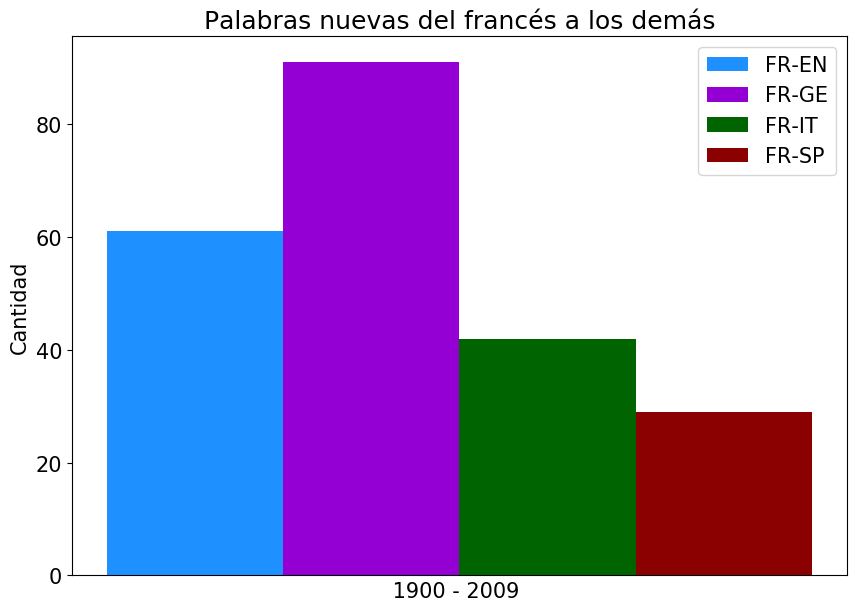
\includegraphics[scale=.4]{Cap_3/ICS_a_FR.png}
				\label{fig.ICS_a_FR}}
		\end{subfigure}
		
		\vspace{0.5cm}
		
		\begin{subfigure}
			[Francés por década.]{
				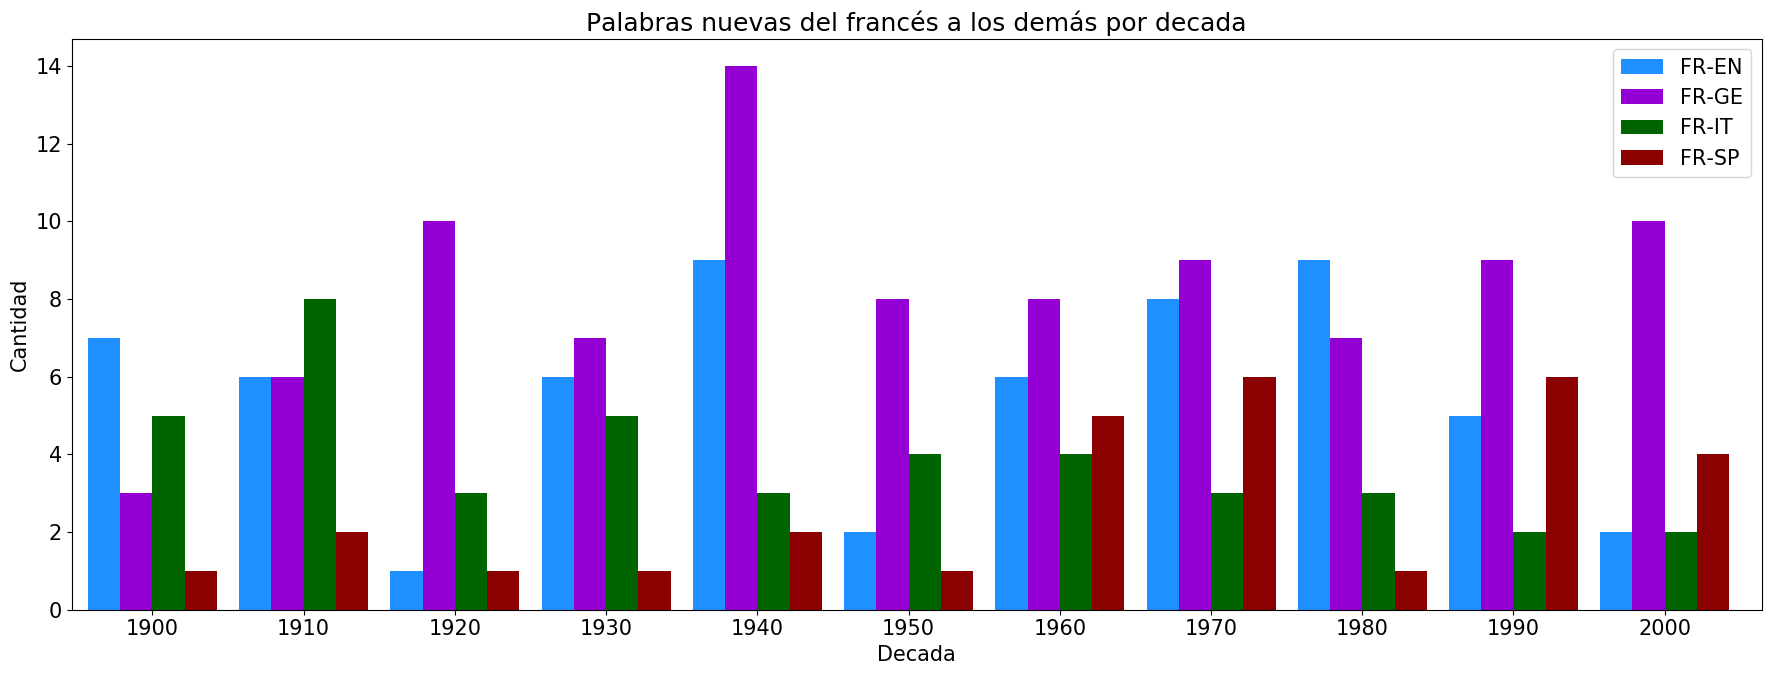
\includegraphics[width=14cm, height=7cm]{Cap_3/ICD_a_FR.png}
				\label{fig.ICD_a_FR}}
		\end{subfigure}
		
		\caption{Palabras nuevas del francés en los demás.}
		\label{fig.IC_FR}
	\end{center}
\end{figure} % }}}


A lo largo del siglo pasado (y primeros años del actual), el alemán se ha
beneficiado de elementos del francés más que los otros, adoptando más del doble
que el español a pesar de ser un idioma de la misma familia. Una posible razón
del por qué el alemán ha sido donde han llegado la mayor cantidad de palabras
es que etimológicamente el francés es más parecido a los otros, y el mayor
aporte a los demás ocurrió antes de 1900.  También es importante destacar que
el papel del francés en 1800 era tan relevante como lo es ahora el inglés,
donde la mayor cantidad de obras eran publicadas en este idioma.

\subsubsection*{Francés-Inglés}% {{{

La característica de los prestamos, es que son principalmente palabras que son comunes en el ingles, y que a simple vista serian catalogados como errores de clasificación, por ejemplo  \textit{diagnostic,} \textit{clients,} \textit{placement,} \textit{adaptation,} \textit{diffusion,} \textit{amplitude,} no pareciese lógico ver que migraron del francés hacia el inglés, sin embargo el algoritmo designo este origen por ser al principio de la base de datos (1740)  donde las palabras eran más utilizadas.  Antes de considerarse un error, se puede inferir que antes las obras en francés eran bastas de vocablos de otros idiomas, destacando el papel que tuvo el francés como idioma "común" para transmitir información. 


% }}}
\subsubsection*{Francés-Alemán}% {{{

De la grafica \ref{fig.ICD_a_FR}, el alemán tuvo dos décadas donde la diferencia de palabras nuevas que llegaron a él es mas significativa que en los otros idiomas, en los periodos de 1920 y 1940  (posteriores a las dos guerras mundiales), entre el contenido se ubicaron a  textit{diplomatie} (1917), \textit{bourgeoisie} (1919),  \textit{guerre} (1925), \textit{Allemagne} (1925), \textit{Russie} (1925) y \textit{empire} (1937); siendo un conjunto de palabras utilizables al referise a temas políticos  o diplomáticos, y por donde participaron países hablantes de las dos lenguas. 


% }}}
\subsubsection*{Francés-Italiano}% {{{

El italiano se vio mas susceptible al francés en los primeros años del siglo, aunque no fue posible ligar a las palabras a un hecho relevante en estos años. Entre las pocas clasificaciones se encuentra la terna cientica con \textit{Poincaré} (1924), apellido del matemático francés Henri Poincaré, y la bélica,  entre los terminos encontrados estan \textit{Versailles} (1924), textit{Vietnam} (1966)  y \textit{URSS} (1975), mostrando que la  La primera y segunda guerra mundial fueron detonantes para el flujo de palabras.


% }}}
\subsubsection*{Francés-Español}% {{{

Al igual que la tendencia en el italiano, en el español no llegaron gran cantidad de palabras cuyo contenido sea ligado a un evento, a pesar de que en cien años migraron alrededor de veinte. La mas destacada fue \textit{euros} (2002) por ser el año de circulación de la moneda de la unión europea, organización donde son miembros países importantes de las dos lenguas. 

El hecho de no poder enlazar palabras a eventos, no significa que el francés no es importante para el español (o el italiano), sino que el periodo donde los hechos tuvieron mayor impacto no esta dentro del periodo de búsqueda,  por ejemplo hechos como la revolución francesa, o la invasión napoleónica a España, propiciaron a un mayor intercambio en este sentido, pero al ocurrir antes de 1900 no permite tener una conclusión de ello. 


% }}}
% }}}
\subsection{Alemán}% {{{

\begin{figure} % {{{
	\begin{center}
		\begin{subfigure}
			[Alemán por siglo.]{
				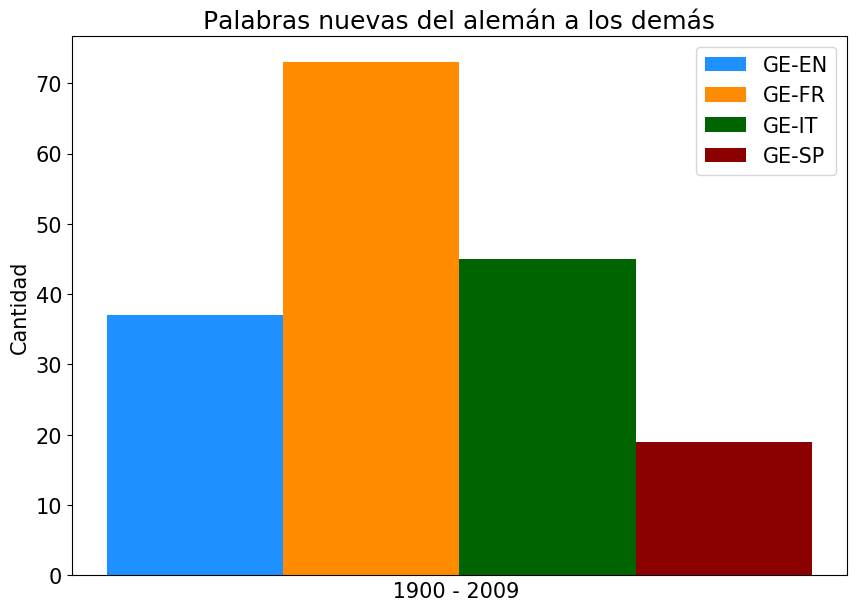
\includegraphics[scale=.4]{Cap_3/ICS_a_GE.png}
				\label{fig.ICS_a_GE}}
		\end{subfigure}
		
		\vspace{0.5cm}
		
		\begin{subfigure}
			[Alemán por década.]{
				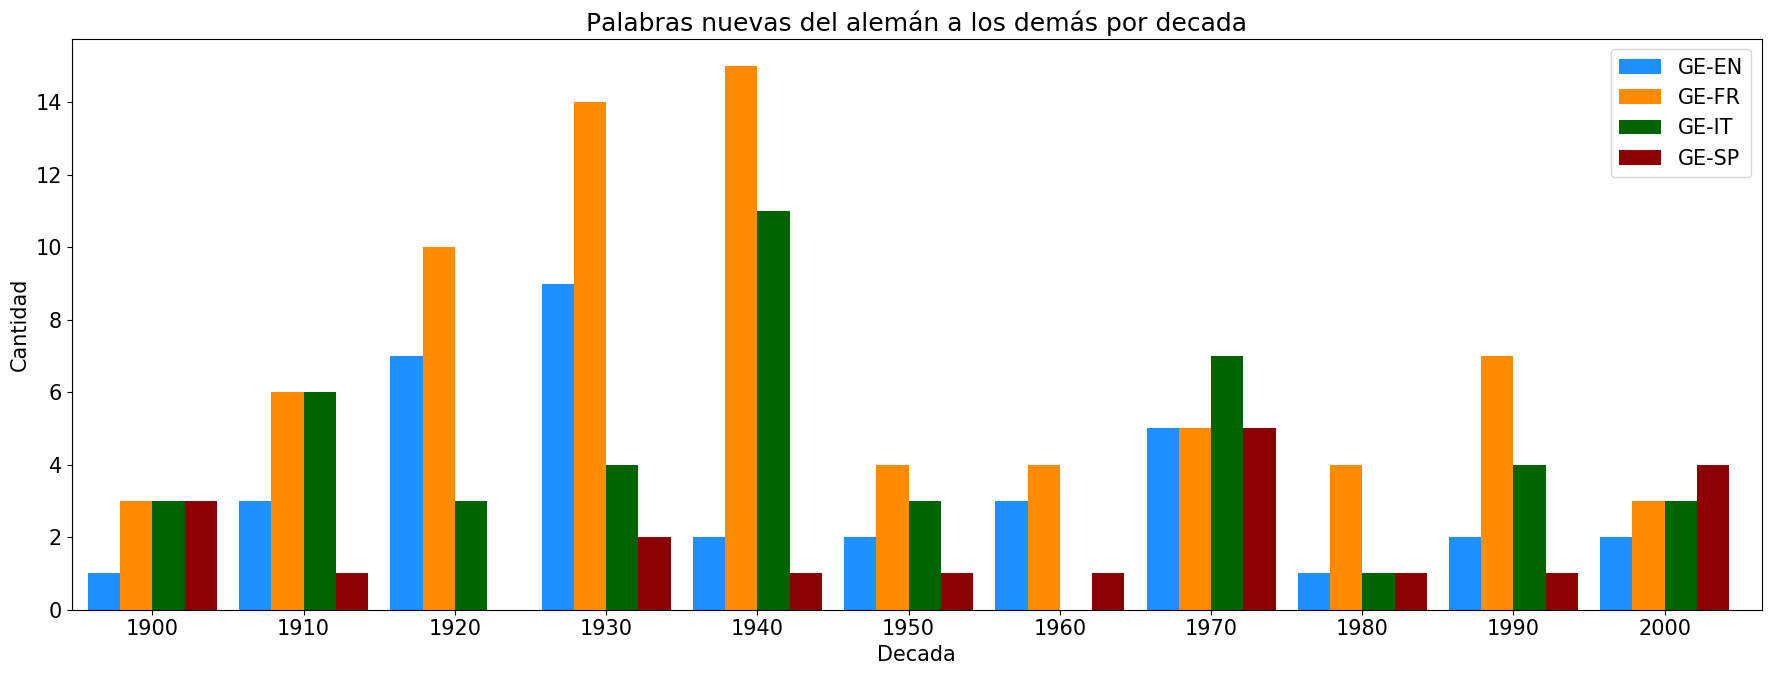
\includegraphics[width=14cm, height=7cm]{Cap_3/ICD_a_GE.png}
				\label{fig.ICD_a_GE}}
		\end{subfigure}
		
		\caption{Palabras nuevas del alemán en los demás.}
		\label{fig.IC_GE}
	\end{center}
\end{figure} % }}}

El principal idioma donde emigraron las palabras del alemán, fue el francés con
casi 70 préstamos, siendo siete veces más que en español, el idioma con menor
cantidad. Destaca el italiano como el segundo con más términos a pesar de que
el inglés proviene de la misma familia de lenguas germánicas.  Campos como el
desarrollo científico, la filosofía  y la política donde los germanoparlantes
tuvieron papeles destacados en el siglo pasado ha hecho posible que las demás
lenguas se impregnan del alemán, y que continuaron usándolos tras la primera
aparición


\subsubsection*{Alemán-Inglés}% {{{

Como en la relación en sentido inverso, en los años posteriores a la segunda guerra mundial,  fueron donde mayores relaciones de palabras se encontraron  \textit{Lenin} (1931), \textit{Hitler} (1934) y \textit{reich} (1939) forman parte  de este contexto histórico.  Otras palabras relevantes son \textit{Marx} (1934) y \textit{Freud}, apellidos de dos personaje sy autores destacados en la filosofía y psicología. 


% }}}
\subsubsection*{Alemán-Francés}% {{{

Como se comento de la grafica por siglo, el francés ha recibido más palabras del alemán que cualquier otro. A pesar de que la mayor cantidad de aportes se dio en la primera mitad de siglo, las relaciones que se encontraron han sido a lo largo de todo el periodo y en diferentes áreas. 

Destaca la década de 1940, con palabras como \textit{regierung},  \textit{deutschen},\textit{minister} y  \textit{bestimmungen}(traducciones de gobierno, alemán, ministro y reglamentos) todas apareciendo en 1944;  si se añaden palabras en años previos como \textit{Hitler} (1933), \textit{kaiser} (1915) y \textit{reich} (1921), son conceptos que muestran parte de la historia del alemán en las guerras. 

El objetivo no es solo identificar sucesos de carácter militar en esta dirección de los préstamos, el identificar un nombre o apellido facilita encontrar las relaciones con un ámbito,  además de Hitler se encontraron los siguientes apellidos:  \textit{Nietzsche} (1905),  \textit{Marx} (1923), \textit{Heidegger} (1987),  \textit{Mozart} (1956), \textit{Freud} (1965) y \textit{Engels} (1970), enlazados a la filosofía, la música y la medicina,  además todos ellos de personajes nacidos en países germanohablantes.


% }}}
\subsubsection*{Alemán-Italiano}% {{{

La proximidad geográfica de Italia con países con lengua oficial en el alemán, hace posible la entrada de palabras, algunas no tan comunes.  Los apellidos de los personajes mencionados anteriormente, también se encuentran en el lenguaje italiano, apareciendo en años próximos a los ya citados.  

El único apellido que se asentó exclusivamente en el  italiano fue \textit{Berchtold} en 1943, aludiendo a Leopold Berchtold ministro de exteriores del Imperio Austro-Húngaro de 1912 a 1915, cuyo fallecimiento ocurrió en 1942.  Se hablo de la proximidad geográfica, ya que este puede ser un factor (ademas del contexto histórico) que detone las migraciones de palabras, la proximidad de Italia con el imperio austro-húngaro puede inferir en la existencia de  palabras que migren entre  dos idiomas y sólo entre ellos. 

  
% }}}
\subsubsection*{Alemán-Español}% {{{

Las palabras que van en este sentido,  presentaron años (o una décadas)  con pocas migraciones o sin alguna, el incremento de palabras se dio posterior a 1950 donde los años sin intercambio disminuyeron.  \textit{Marx} (1932), \textit{kaiser} (1938), \textit{Hitler} (1940), \textit{Lenin} (1970), \textit{Hegel} (1971),  \textit{Nietzsche} (2000) y \textit{Freud} (2002) son parte de los términos que llegaron al español,  sin embargo, es peculiar que las dos últimas hayan aparecido en el español muchos años después que en los demás idiomas, por ejemplo en el francés,  Nietzsche apareció 1905 y Freud en 1965. El letargo de años puede ser una característica del tiempo que les lleva  a las  palabras del alemán pasar hacia el español, al adaptarse a una lengua de una familia distinta y donde históricamente no ha existido un evento conjunto entre países. 



% }}}
% }}}
\subsection{Italiano}% {{{

\begin{figure} % {{{
	\begin{center}
		\begin{subfigure}
			[Italiano por siglo.]{
				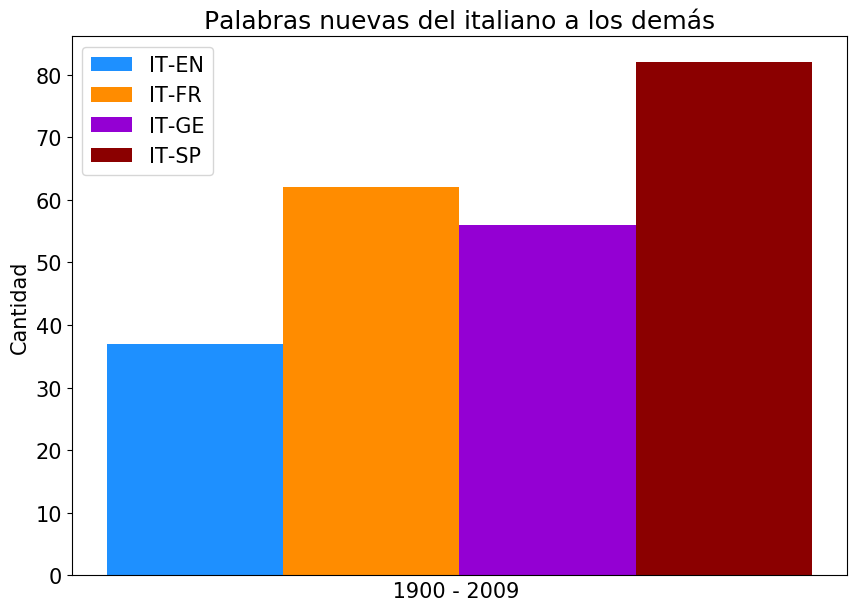
\includegraphics[scale=.4]{Cap_3/ICS_a_IT.png}
				\label{fig.ICS_a_IT}}
		\end{subfigure}
		
		\vspace{0.5cm}
		
		\begin{subfigure}
			[Italiano por década.]{
				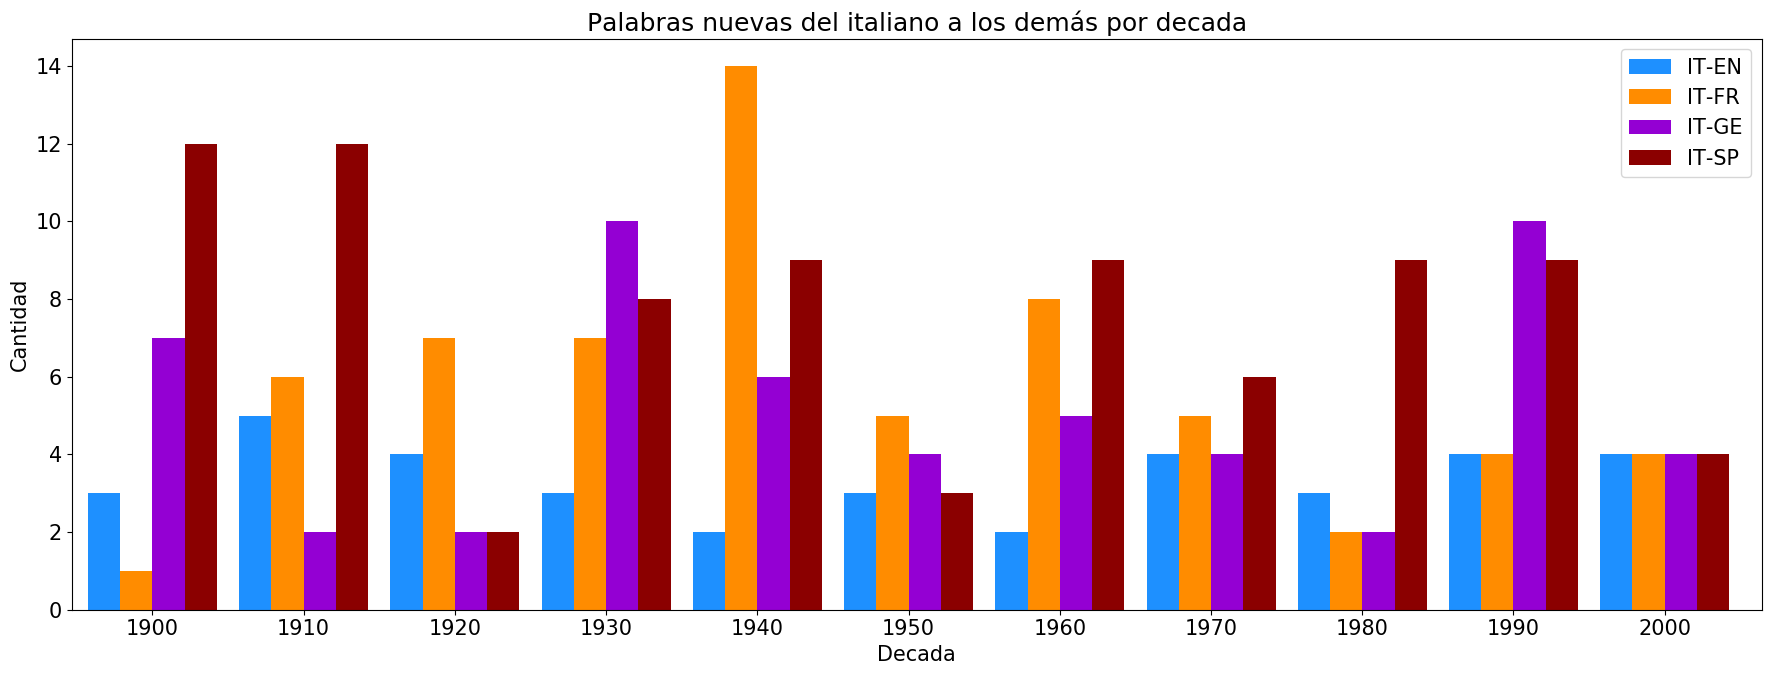
\includegraphics[width=14cm, height=7cm]{Cap_3/ICD_a_IT.png}
				\label{fig.ICD_a_IT}}
		\end{subfigure}
		
		\caption{Palabras nuevas del italiano en los demás.}
		\label{fig.IC_IT}
	\end{center}
\end{figure} % }}}


Por ser lenguajes parecidos fonética y etimológicamente al provenir de la misma
raíz grecolatina,  el español ha adoptado la mayor cantidad de palabras
provenientes del italiano,  seguido del francés otra lengua romance.  

\subsubsection*{Italiano-Inglés}% {{{

A pesar de que en cada década existen términos nuevos en el inglés, solo ha sido posible asociar \textit{mussolini} (1935) al político y militar Benito Mussolini, tal vez el personaje italiano más relevante para la historia en el siglo XX 

% }}}
\subsubsection*{Italiano-Francés}% {{{



En las migraciones sólo se asoció \textit{Mussolini} (1935), la cual ya se había mencionado en las migraciones del italiano al inglés, tras revisar las listas de migraciones con origen italiano  a los demás idiomas, Mussolini siempre se encuentra en todas las migraciones y en el mismo año ratificando la importancia de este término en la historia. 

Aunque en 1940 migraron la mayor cantidad de préstamos, ninguno de ellos ha tenido contexto con los sucesos de esa época. 

% }}}
\subsubsection*{Italiano-Alemán}% {{{

En esta dirección de las palabras del italiano, si fue posible relacionarlas con el contexto bélico,  \textit{regime} (1938), \textit{panzer} (1941), \textit{duce} (1942),  traducciones de régimen, blindado y líder, además de \textit{Mussolini} (1935). 



% }}}
\subsubsection*{Italiano-Español}% {{{

En el español, las tendencias no fueron sólo hacia la guerra, también a idelogías políticas como \textit{socialista} (1914), \textit{comunista} (1932), \textit{capitalismo} (1935), \textit{fascismo} (1937),  \textit{marxismo} (1963) y \textit{terrorismo} (1986). 



% }}}
% }}}
\subsection{Español}% {{{

\begin{figure} % {{{
	\begin{center}
		\begin{subfigure}
			[Español por siglo.]{
				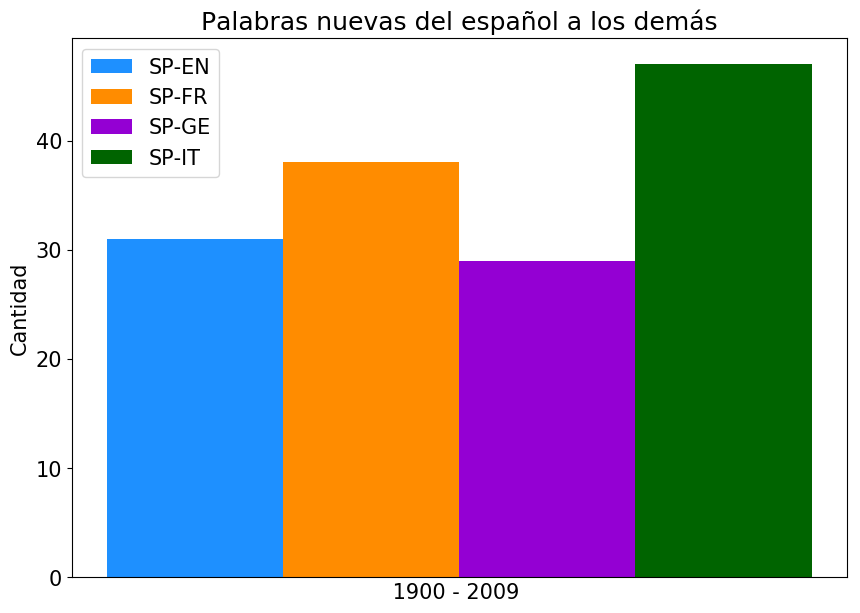
\includegraphics[scale=.4]{Cap_3/ICS_a_SP.png}
				\label{fig.ICS_a_SP}}
		\end{subfigure}
		
		\vspace{0.5cm}
		
		\begin{subfigure}
			[Español por década.]{
				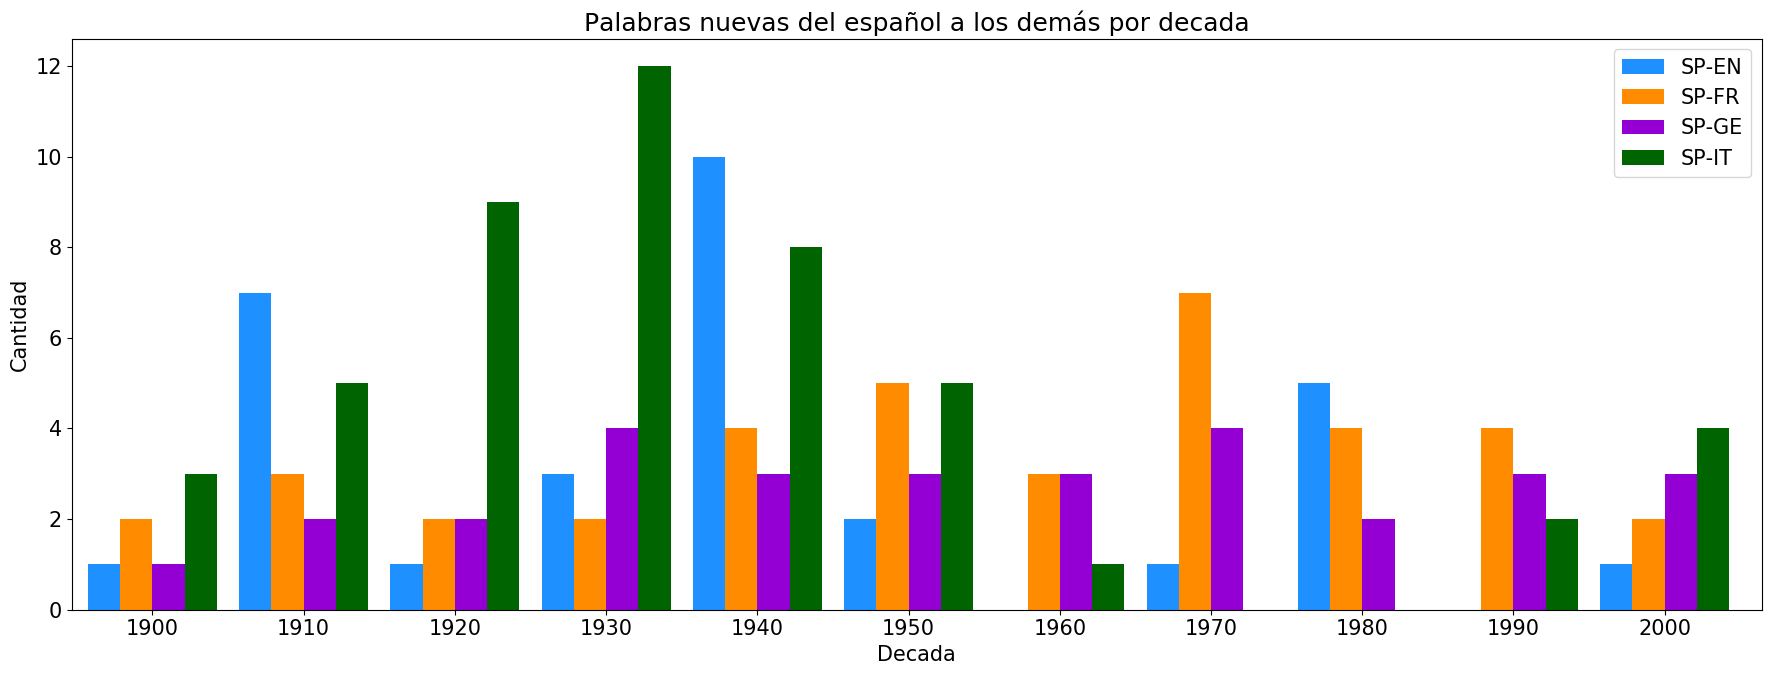
\includegraphics[width=14cm, height=7cm]{Cap_3/ICD_a_SP.png}
				\label{fig.ICD_a_SP}}
		\end{subfigure}
		
		\caption{Palabras nuevas del español en los demás.}
		\label{fig.IC_SP}
	\end{center}
\end{figure} % }}}

Entre todas las combinaciones de idioma origen e idioma receptor,  la relación
entre el español y el italiano, es la única reciproca, donde  el italiano ahora
es el que más palabras recibió del español (anteriormente que el idioma que mas
presencia tuvo en el español fue el italiano).  Nuevamente la otra lengua
romance, el francés es la segunda que mas términos adopto,  mientras que las
germánicas las de menor impacto.  La composición de las etimologías de un
idioma son un factor para que algún otro se adapte en él, es mas sencillo que
existan migraciones entre lenguajes de la misma familia. 

\subsubsection*{Español-Inglés}% {{{

Resalta que hay décadas donde el aporte al inglés es mínimo (o no existe). Contrario a la tendencia en las anteriores migraciones donde la guerra era una constante para que se diese el flujo de palabras, en este sentido se encontraron términos médicos en el año de 1943 (la decadas mas prolifera del español en el inglés) aparecieron las palabras \textit{virus} y \textit{anemia}, años antes en 1934 George Richards Minot, Parry Murphy y George Hoiyt Whipple, habían recibido el premio nobel de medicina por su descubrimiento de la terapia de hígado para el tratamiento de anemias.   

Probablemente las palabras virus y anemia ya existían en el inglés años antes de 1943,  pero sólo hasta este año tuvieron la importancia para estar dentro de las cinco mil mas utilizadas. Con este ejemplo, se trata se ver que hay eventos (como un premio internacional) que retoman palabras cuo periodo de uso  ha disminuido y las vuelve a impulsar para distribuirse en los demás idiomas.   No siempre serán las palabras mas recientes en el origen las que realicen las migraciones. 

% }}}
\subsubsection*{Español-Francés}% {{{

El primer préstamo que resultó importante del español hacia el francés es \textit{Panamá} (1913), su trascendencia se liga al año de inauguración del canal de Panamá en 1914, siendo una obra importante para el comercio de la época al conectar los océanos pacífico y atlántico, además el primer gobierno que impulsó económicamente la construcción del canal fue el francés,  aunque su conclusión y administración pasó a los Estados Unidos.  




% }}}
\subsubsection*{Español-Alemán}% {{{


La investigación hecha para ligar muestran nuevamente términos médicos, la palabra \textit{lepra} (1901) fue globalmente importante a partir de 1874,  ya que en ese año el científico noruego Gerhard Armauer Hansen descubrió el bacilo de Hansen Mycobacterium Leprae \cite{lepra} que origina la enfermedad. Por el carácter médico de la palabra es probable que se hiciera más investigación sobre la enfermedad en diferentes idiomas, en este caso el alemán.

Como en las migraciones hacia el ingles, son términos que vuelven a ser importantes,  y esto les permite migrar a otros idiomas. 


% }}}
\subsubsection*{Español-Italiano}% {{{

Los términos médicos han sido una constante en las migraciones del español,en el italiano se encontraron \textit{virus} (1922), \textit{colesterina} (1928),  \textit{sintomatología} (1931), \textit{anestesia} (1932), \textit{vitamina} (1935), \textit{anemia} (1936), \textit{metabolismo} (1936) y \textit{gástrica} (1936)  y \textit{endovenosa} (1937).  

El aparecer estas palabras en el español (dentro de las cinco mil más usadas)antes que en los demás propone que la medicina era un campo importante para los países de habla española, donde posiblemente en los años del conjunto base (1740-1900) se publicaron más libros de medicina en lenguaje español. 





\hfill\break
\hfill\break

% }}}
% }}}
% }}}
\section{Comentarios del método}% {{{


Tras las múltiples combinaciones entre idiomas, se  encontró que el principal
evento que origino las migraciones ha sido la segunda guerra mundial donde
todos los lenguajes recibieron un termino asociado a ella durante el siglo XX.

Se destaca el papel del inglés en las ultimas dos décadas como el idioma común
para transmitir información; además de ser el exportador de palabras en campos
como la tecnología, disciplina que ha hecho posible la fluidez con la que se
mueve a información. El poderío económico ha hecho de países como los Estados
Unidos una fuente de nueva información.

El alemán también ha acaparado las migraciones, se han distinguido dos causas
de la importancia de este idioma tanto como origen como receptor, la primera
por el papel representado en la historia del siglo XX principalmente por
Alemania donde la guerra permitió la comunicación de varias lenguas con el
alemán, incluso después de que estas terminara, así mismo el protagonismo de
personajes germanoparlantes en diferentes áreas ha hecho que el alemán se
expanda incluso en lenguajes que no son de su propia familia lingüística. 

Finalmente entre las tres lenguas romances, aunque no hayan sido tan
protagonistas (no aporten palabras con un contenido afín),  su periodo de
apogeo e influencia hacia los demás no se tiene registrado en este trabajo.
Destacan los conceptos médicos en la lengua española, mostrando la importancia
que tenia la medicina y la cantidad de libros que se publicaban en esta área en
este idioma. 

Entre las principales deficiencias del método, es que aun es ambiguo decir
quien ha influido mas en los otros; por el momento sólo se puede decir la
manera en que se ha reflejado la influencia, cada conjunto de palabras que
migraron de un idioma a otro, tienen relación a algún ámbito, la guerra, la
economía, la tecnología, las ciencias, las artes y la medicina; cada
combinación tendrá mas elementos de alguna de estas áreas.  Se realizara otro
método para cuantificar la influencia de unos sobre otros. 

% }}}

